\scanpage{11}
$T$ torseur \unsure{:|à} droite sous \unsure{grp|grpe} $\unsure{\mathbb{Z}|Z}$

\[
\deleted{\unsure{\operatorname{Aut}_{\substack{G\text{-ens}\\G\text{-}\unsure{\mathrm{var}|\mathrm{op}}}}(\unsure{D|T})
 \longrightarrow\operatorname{Aut}(G)}}
\]

\diagram{\begin{tikzcd}[ampersand replacement=\&,column sep=small]
1\arrow[r] \& \mathbb{Z}\arrow[r,"i"] \& \operatorname{Aut}(\mathbb{Z},T)\arrow[r,"p"]
 \& \operatorname{Aut}(\mathbb{Z})\arrow[r,dash]\arrow[l,dashed,bend left=28,"q_t"'] \& 1
\end{tikzcd}}

% A detached short dark mark stands above un; ink versus surface trace is unresolved.
$\forall t\in T$, on a \tikz[baseline=(wordun.base)]{
\node[anchor=base west,inner sep=0pt] (wordun) at (0,0) {un};
\node[inner sep=0pt] at (.30,.42) {\unsure{\tikz[baseline=-.2ex]{\draw[line width=.6pt,line cap=round] (0,0)--(.05,0);}}};}
splitting $q_t$, défini par
\[
\left\{\begin{aligned}&q_t(\gamma)(t)=t\\&p(q_t(\gamma))=\gamma\end{aligned}\right.
\]

Quelle est la relation entre $q_t$ et $q_{t'}$ ?

On \unsure{avait|aurait} $t'=t.g$, et on trouve
\[
q_{t'}=\operatorname{int}(i(g))\circ q_t
 \;:\; \gamma\longrightarrow i(g)\,q_t(\gamma)\,i(g)^{-1}
\]

[ Pour le vérifier, il suffit de voir que
% The brace starts after int, ends below q_t, and has a displaced slanting equals below it.
\[
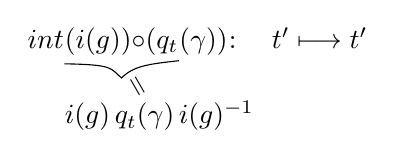
\begin{tikzpicture}[baseline=(proofint.base)]
\node[anchor=base west,inner sep=0pt] (proofint) at (0,0) {$\operatorname{int}$};
\node[anchor=base west,inner sep=0pt] (proofarg) at (proofint.base east) {$(i(g))\unsure{\circ}(q_t$};
\node[anchor=base west,inner sep=0pt] (prooftail) at (proofarg.base east) {$(\gamma))$};
\node[anchor=base west,inner sep=0pt] at (prooftail.base east) {$:\quad t'\longmapsto t'$};
\draw ([yshift=-.10cm]proofarg.south west)
 .. controls +(.65cm,-.01cm) and +(-.15cm,.12cm) .. ([yshift=-.28cm]proofarg.south)
 .. controls +(.15cm,.16cm) and +(-.35cm,-.04cm) .. ([yshift=-.06cm]proofarg.south east);
\node[inner sep=0pt,rotate=-60] at ([xshift=.18cm,yshift=-.40cm]proofarg.south) {$=$};
\node[anchor=north west,inner sep=0pt] at ([yshift=-.57cm]proofarg.south west)
 {$i(g)\,q_t(\gamma)\,i(g)^{-1}$};
\end{tikzpicture}
\]
or \quad $t'=tg$
\[
\begin{aligned}
&\deleted{q_t(\gamma)(t')=q_t(\gamma)(t)\,\gamma(g)=t.\gamma(g)}\\
&\hspace{.3em}\deleted{\operatorname{int}(i(g))\,q_t(\gamma)\,(t')=}\\
&\quad i(g)^{-1}(t')=t\qquad q_t(\gamma)\,i(g)^{-1}(t')=q_{\unsure{b|t}}(\gamma)\,t=t\\
&\qquad i(g)\,q_t(\gamma)\,i(g)^{-1}(t')=tg=t'\qquad\text{ok}\qquad ]
\end{aligned}
\]

\reversemarginpar
\margin{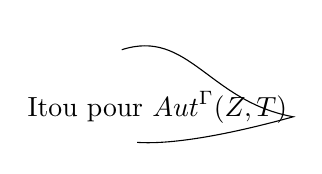
\begin{tikzpicture}[x=.65cm,y=.65cm,baseline=(itou.base)]
\node[anchor=west,inner sep=0pt] (itou) at (0,0) {Itou pour $\operatorname{Aut}^{\Gamma}(\mathbb{Z},T)$};
\draw (1.85,1.13) .. controls (3.15,1.55) and (3.55,.12) .. (5.20,-.18)
 .. controls (4.05,-.50) and (2.88,-.73) .. (2.15,-.68);
\end{tikzpicture}}
\normalmarginpar

% Ex and Z=Z_n are on the baseline of the lower (Aut) row; the canceled fragment lies beneath Z=Z_n.
\[
\begin{aligned}
&\text{\uline{Ex}}\quad \mathbb{Z}=\mathbb{Z}_n\quad
\left\{\begin{aligned}[b]
\operatorname{End}\mathbb{Z}&=\mathbb{Z}_n\\
\operatorname{Aut}\mathbb{Z}&=\mathbb{Z}_n^{*}\supset\{\pm1\}=\Gamma
\end{aligned}\right.\\
&\hspace{3.8em}\deleted{\unsure{\Gamma\in|\Gamma\subset}}
\end{aligned}
\]
\margin{(\uline{NB} \unsure{si} $n=2$, $+1=-1$ dans $\mathbb{Z}_n^{*}$\ldots)}

\[
\begin{aligned}
&\operatorname{Aff}(\mathbb{Z}_n)=\mathbb{Z}_n\mathbin{.}\mathbb{Z}_n^{*}
 \quad\text{(produit ${}^1\! /\! {}_2$ direct)}
 \quad\raisebox{.7em}{\unsure{\tikz[baseline=0pt]{\fill (0,0) circle (.4pt);\fill (.05,.075) circle (.4pt);}}}\\[-.3em]
&\text{\llap{\tikz[baseline=-.1ex]{\draw[line width=.7pt,line cap=round] (0,.04)--(0,0)--(.025,0);}\hspace{1.6em}}}
 \hspace{1.7em}\rotatebox{90}{$\subset$}\\[-.3em]
&\hspace{.5em}\operatorname{Aff}^{\{\pm1\}}(\mathbb{Z}_n)=\mathbb{Z}_n\mathbin{.}\{\pm1\}
\end{aligned}
\]
% The upper-right points have uncertain writing status. The separate lower-left stroke is drawn without assigned function.
\margin{groupe diédral d'indice $n$, $\mathbb{D}_n$ (on suppose $n\ne2$\ldots)}

Soit $T$ torseur sous $Z$ groupe cyclique d'ordre $n\geq3$ muni d'une famille $\{u,u^{-1}\}$ de 2 gén. \tikz[baseline=(old.base)]{
\node[anchor=base west,inner sep=0pt] (old) at (0,0) {\deleted{\unsure{d'ordre $n$}.}};
\node[anchor=south west,inner sep=0pt] at ([yshift=.14em]old.north west)
 {\inserted{inverses l'un de l'}};}autre.
\diagram{\begin{tikzcd}[ampersand replacement=\&,column sep=small]
1\arrow[r] \& Z\arrow[r,dash,"i"] \& \operatorname{Aut}^{\pm1}(T,Z)\arrow[r,dash,"p"]
 \& \{\pm1\}\arrow[r,dash]\arrow[l,bend left=25,"q"{auto=false,inner sep=0pt}] \& 1
\end{tikzcd}}
% archive sheet number: 10
